\documentclass[11pt,a4paper]{article}
\usepackage[margin=2.3cm]{geometry}
\usepackage[T1]{fontenc}
\usepackage[utf8]{inputenc}
\usepackage{lmodern}
\usepackage{xcolor}
\usepackage{graphicx}
\usepackage{amsmath,amssymb}
\usepackage{booktabs,array,longtable}
\usepackage{listings}
\usepackage[most]{tcolorbox}
\usepackage{caption}
\usepackage{tikz}
\usetikzlibrary{arrows.meta,positioning,shapes.geometric,fit,backgrounds}
\usepackage{pgfplots}
\pgfplotsset{compat=1.18}
\usepackage{microtype}
\usepackage{enumitem}
\usepackage{fancyhdr}
\usepackage[colorlinks=true,linkcolor=cProcess,urlcolor=cInput,citecolor=cProcess]{hyperref}

% ---------- Semantic palette (cool "systems" blues + one warm accent) ----------
\definecolor{cInput}{HTML}{2E6F8E}    % source programs, files you give the tools
\definecolor{cProcess}{HTML}{1F3A5F}  % compiler stages: lexer, parser, AST, emitter
\definecolor{cResult}{HTML}{C2703D}   % outputs: program output, executables, answers
\definecolor{cAlert}{HTML}{A63A50}    % warnings, limitations, things that break
\definecolor{cNeutral}{HTML}{5B6472}  % arrows, labels, structure
\definecolor{cBg}{HTML}{F2F4F7}       % panel / code backgrounds

\setlist{itemsep=2pt,topsep=4pt}
\setlength{\parindent}{0pt}
\setlength{\parskip}{5pt}

\pagestyle{fancy}
\fancyhf{}
\fancyhead[L]{\small\color{cNeutral}KiteLang -- README}
\fancyhead[R]{\small\color{cNeutral}\thepage}
\renewcommand{\headrulewidth}{0.4pt}

\captionsetup{font=small,labelfont={bf,color=cProcess}}

% ---------- Code listings ----------
\lstdefinelanguage{Kite}{
  morekeywords={int,float,bool,void,return,print,true,false},
  morekeywords=[2]{pecha,warna,dheel,dor,palta},
  sensitive=true, morecomment=[l]{//}
}
\lstset{
  basicstyle=\ttfamily\small, backgroundcolor=\color{cBg},
  frame=single, rulecolor=\color{cNeutral!40}, framesep=4pt,
  breaklines=true, columns=fullflexible, keepspaces=true,
  keywordstyle=\color{cProcess}\bfseries,
  keywordstyle=[2]\color{cInput}\bfseries,
  commentstyle=\color{cNeutral}\itshape,
  showstringspaces=false, aboveskip=6pt, belowskip=6pt
}
\lstnewenvironment{shell}{\lstset{language=bash,keywordstyle=\color{black}}}{}
\lstnewenvironment{kite}{\lstset{language=Kite}}{}
\lstnewenvironment{outtext}{\lstset{backgroundcolor=\color{cResult!8},rulecolor=\color{cResult!60}}}{}

% ---------- Role boxes ----------
\newtcolorbox{defbox}[1][]{colback=cProcess!5,colframe=cProcess!70,fonttitle=\bfseries\small,title={#1},boxrule=0.6pt,arc=2pt}
\newtcolorbox{resultbox}[1][]{colback=cResult!8,colframe=cResult,fonttitle=\bfseries\small,title={#1},boxrule=0.6pt,arc=2pt}
\newtcolorbox{warnbox}[1][]{colback=cAlert!6,colframe=cAlert,fonttitle=\bfseries\small,title={#1},boxrule=0.6pt,arc=2pt}

\newcommand{\kw}[1]{\texttt{\textcolor{cInput}{\textbf{#1}}}}
\newcommand{\fn}[1]{\texttt{#1}}

\begin{document}

% ---------- Title ----------
\begin{titlepage}
\centering
\vspace*{2.5cm}
{\color{cProcess}\Huge\bfseries KiteLang\par}
\vspace{0.4cm}
{\Large A Basant-inspired language with a Flex/Bison interpreter\\ and an LLVM Ahead-of-Time compiler\par}
\vspace{0.8cm}
{\large\color{cNeutral} Compiler Construction -- Course Project\\ README: build, run and usage guide for Linux\par}
\vspace{1.8cm}
\begin{tabular}{ll}
\toprule
\textbf{Group member} & \textbf{Roll number}\\
\midrule
Mohammad Ibrahim Salman & 23L-0723\\
Muzammil Ahmed Bhatti & 23L-0688\\
Muhammad Ali Mahoon & 23L-0531\\
\bottomrule
\end{tabular}
\vfill

\begin{tikzpicture}
\fill[cInput!80] (0,1) -- (0.7,0) -- (0,-1) -- (-0.7,0) -- cycle;
\draw[cProcess,thick] (0,1) -- (0,-1) (-0.7,0) -- (0.7,0);
\draw[cNeutral,thick] (0,-1) .. controls (0.4,-1.6) and (-0.4,-2) .. (0.1,-2.6);
\end{tikzpicture}
\vspace{1cm}
\end{titlepage}

\tableofcontents
\newpage

% =====================================================================
\section{Quick start (for the grader)}

If you only want to check that both phases work, run these commands from the project root on Ubuntu/Debian:

\begin{shell}
sudo apt update
sudo apt install -y build-essential flex bison clang llvm
make            # builds both phases into build/
make test       # runs Phase 1 and Phase 2 and compares output
\end{shell}

\begin{resultbox}[What success looks like]
\fn{make test} prints no \fn{diff} output and exits with status 0. That means the interpreter \emph{and} the natively compiled program both printed \fn{1 2 4 7 8 9} (one number per line), which matches \fn{tests/expected\_insertion\_sort.txt}.
\end{resultbox}

The rest of this guide explains every step in detail.

% =====================================================================
\section{What KiteLang is}

KiteLang is a small language for writing algorithm programs. It is inspired by \emph{Basant}, the kite-flying festival. It keeps C-style functions, variables, arrays, expressions and braces, and replaces the control-flow keywords with kite-flying words:

\begin{center}
\begin{tabular}{>{\ttfamily}l l}
\toprule
\textrm{\textbf{Keyword}} & \textbf{Meaning}\\
\midrule
\kw{pecha} & \texttt{if}\\
\kw{warna} & \texttt{else}\\
\kw{dheel} & \texttt{while}\\
\kw{dor}   & inclusive, increasing range loop\\
\kw{palta} & swap two assignable values\\
\bottomrule
\end{tabular}
\end{center}

The project implements both required phases:

\begin{enumerate}
\item \textbf{Phase 1 -- Interpreter.} Flex splits the source into tokens. Bison checks the grammar and builds an AST. C++ code inside the Bison grammar file then executes that AST directly. No intermediate code is produced.
\item \textbf{Phase 2 -- AOT compiler.} The same parser turns the AST into textual LLVM IR (a \fn{.ll} file). Clang compiles that IR into a native Linux executable.
\end{enumerate}

\begin{defbox}[Terms used in this guide]
\begin{itemize}[leftmargin=*]
\item \textbf{Lexer (Flex):} reads raw text and cuts it into \emph{tokens}, the ``words'' of the language, such as \kw{dor}, \fn{42} or \fn{+}.
\item \textbf{Parser (Bison):} checks that the tokens follow the grammar rules and builds a tree from them.
\item \textbf{AST (Abstract Syntax Tree):} a tree that represents the program's structure, e.g.\ ``an \fn{if} node with a condition child and a body child''.
\item \textbf{Interpreter:} a program that walks the AST and performs each action immediately.
\item \textbf{LLVM IR:} LLVM's portable, assembly-like \emph{intermediate representation}. Clang can turn it into machine code.
\item \textbf{AOT (Ahead-of-Time) compiler:} translates the whole program into an executable \emph{before} it runs.
\end{itemize}
\end{defbox}

Figure~\ref{fig:pipeline} shows how the two phases share the front end and split after the AST.

\begin{figure}[ht]
\centering
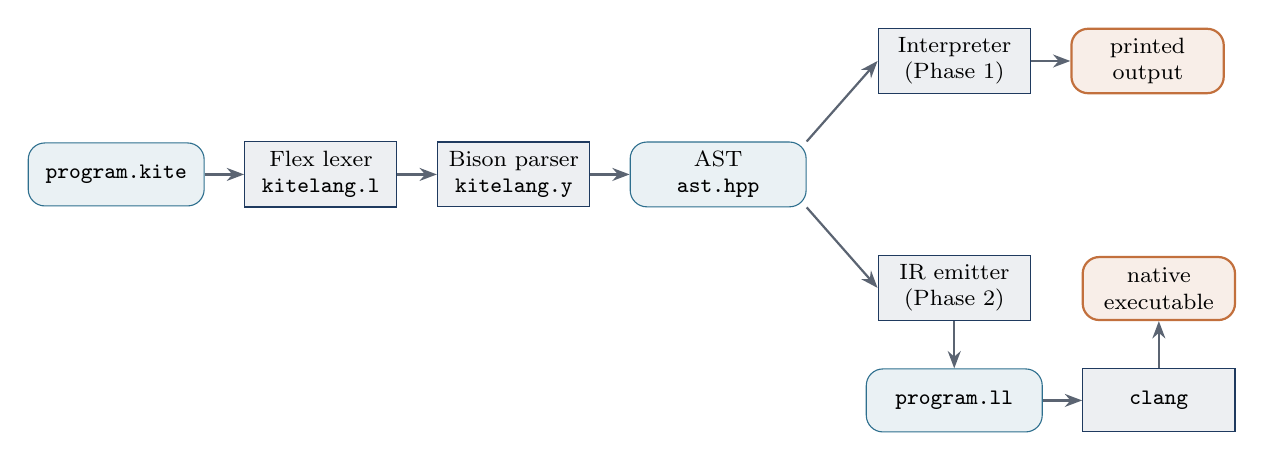
\begin{tikzpicture}[
  font=\footnotesize, node distance=6mm and 5mm,
  data/.style={draw=cInput,fill=cInput!10,rounded corners=6pt,minimum height=8mm,align=center,text width=20mm},
  stage/.style={draw=cProcess,fill=cProcess!8,minimum height=8mm,align=center,text width=17mm},
  outn/.style={draw=cResult,fill=cResult!12,rounded corners=6pt,minimum height=8mm,align=center,text width=17mm,thick},
  arr/.style={-{Stealth[length=2.2mm]},cNeutral,thick}]
\node[data]  (src) {\fn{program.kite}};
\node[stage, right=of src] (lex) {Flex lexer\\\fn{kitelang.l}};
\node[stage, right=of lex] (par) {Bison parser\\\fn{kitelang.y}};
\node[data,  right=of par] (ast) {AST\\\fn{ast.hpp}};
\node[stage, above right=6mm and 9mm of ast] (int) {Interpreter\\(Phase 1)};
\node[outn, right=of int] (o1) {printed\\output};
\node[stage, below right=6mm and 9mm of ast] (ir) {IR emitter\\(Phase 2)};
\node[data,  below=of ir] (ll) {\fn{program.ll}};
\node[stage, right=of ll] (cl) {\fn{clang}};
\node[outn, above=of cl] (exe) {native\\executable};
\draw[arr] (src)--(lex); \draw[arr] (lex)--(par);
\draw[arr] (par)--(ast);
\draw[arr] (ast.north east)--(int.west); \draw[arr] (int)--(o1);
\draw[arr] (ast.south east)--(ir.west); \draw[arr] (ir)--(ll); \draw[arr] (ll)--(cl); \draw[arr] (cl)--(exe);
\end{tikzpicture}
\caption{Both phases share the Flex lexer, Bison parser and AST. Phase 1 executes the AST directly; Phase 2 writes LLVM IR, which Clang turns into a native program. Rounded = data, square = processing step, orange = final output.}
\label{fig:pipeline}
\end{figure}

% =====================================================================
\section{Installing dependencies (Linux)}

You need \fn{make}, a C++17 compiler (\fn{g++}), Flex, Bison, Clang and LLVM. On Ubuntu/Debian:

\begin{shell}
sudo apt update
sudo apt install -y build-essential flex bison clang llvm
\end{shell}

Check that the tools are installed:

\begin{shell}
flex --version
bison --version
g++ --version
clang --version
\end{shell}

\begin{warnbox}[Clang version]
The generated IR uses LLVM's \emph{opaque pointer} type \fn{ptr}. Use \textbf{Clang/LLVM 15 or newer}. Ubuntu 24.04 ships a new enough Clang by default. On an older release (for example Ubuntu 22.04, which defaults to Clang 14), install a newer version and use it in the Phase 2 commands:
\begin{shell}
sudo apt install -y clang-15
clang-15 build/insertion.ll -o build/insertion
\end{shell}
\fn{make test} calls plain \fn{clang}, so on such a system either make \fn{clang} point to the newer version or run the Phase 2 steps by hand (Section~\ref{sec:phase2}).
\end{warnbox}

% =====================================================================
\section{Compiling the project}

From the project root:

\begin{shell}
make
\end{shell}

This builds two programs from the same source files. The only difference is a preprocessor flag:

\begin{center}
\begin{tabular}{l l l}
\toprule
\textbf{Executable} & \textbf{Phase} & \textbf{Built with flag}\\
\midrule
\fn{build/kitelang-interpreter} & 1 -- interpreter & \fn{-DMODE\_INTERPRETER}\\
\fn{build/kitelang-compiler}    & 2 -- AOT compiler & \fn{-DMODE\_COMPILER}\\
\bottomrule
\end{tabular}
\end{center}

What \fn{make} does, step by step:
\begin{enumerate}
\item Creates the \fn{build/} directory.
\item Runs \fn{bison -d -o build/parser.tab.cpp src/kitelang.y}. This produces the parser and its header \fn{build/parser.tab.hpp}.
\item Runs \fn{flex -o build/lex.yy.cpp src/kitelang.l} to produce the lexer.
\item Compiles both generated files with \fn{g++ -std=c++17 -Wall -Wextra -O2}, once for each mode.
\end{enumerate}

All Makefile targets:

\begin{center}
\begin{tabular}{l l}
\toprule
\textbf{Command} & \textbf{Effect}\\
\midrule
\fn{make} & build both phases\\
\fn{make interpreter} & build Phase 1 only\\
\fn{make compiler} & build Phase 2 only\\
\fn{make test} & build and verify both phases end to end\\
\fn{make clean} & delete the \fn{build/} directory\\
\bottomrule
\end{tabular}
\end{center}

The variables \fn{FLEX}, \fn{BISON}, \fn{CXX} and \fn{CXXFLAGS} can be overridden, e.g.\ \fn{make CXX=clang++}.

% =====================================================================
\section{Running a KiteLang program}

\subsection{Phase 1 -- Interpreter}

\begin{shell}
./build/kitelang-interpreter examples/insertion_sort.kite
\end{shell}

Expected output:

\begin{outtext}
1
2
4
7
8
9
\end{outtext}

The interpreter parses the file and runs \fn{main} straight away. The value \fn{main} returns becomes the process exit status (\fn{return 0;} gives exit code 0). You can check it with \fn{echo \$?}.

\subsection{Phase 2 -- AOT compiler}
\label{sec:phase2}

\begin{shell}
./build/kitelang-compiler examples/insertion_sort.kite -o build/insertion.ll
clang build/insertion.ll -o build/insertion
./build/insertion
\end{shell}

\begin{enumerate}
\item The first command parses the program, writes LLVM IR to \fn{build/insertion.ll} and prints \fn{generated build/insertion.ll}. If you leave out \fn{-o}, the IR goes to \fn{out.ll} in the current directory.
\item The second command uses Clang to compile the IR into a native executable.
\item The third command runs that executable. It prints the same six numbers as the interpreter.
\end{enumerate}

Every generated \fn{.ll} file starts with a format string and a declaration of C's \fn{printf}, which \kw{print} uses:

\begin{lstlisting}
@fmt = private constant [4 x i8] c"%d\0A\00"
declare i32 @printf(ptr, ...)
\end{lstlisting}

Each KiteLang function then becomes one \fn{define i32} (or \fn{define void}) function. Integer parameters are \fn{i32} and array parameters are \fn{ptr}.

\subsection{Command-line usage}

\begin{shell}
kitelang-interpreter source.kite
kitelang-compiler   source.kite [-o output.ll]
\end{shell}

If you run either tool with no arguments, it prints a usage message and exits with status 2. A file that cannot be opened also gives status 2. A syntax error gives status 1.

% =====================================================================
\section{Using the language}

\subsection{Program structure and functions}

A program is one or more functions and must include \fn{main}. Parameters are C-style, and array parameters are written with \fn{[]}. Recursion is supported.

\begin{kite}
int add(int left, int right) {
    return left + right;
}

void show(int values[], int count) {
    dor (i : 0 -> count - 1) {
        print(values[i]);
    }
}

int main() {
    print(add(2, 3));
    return 0;
}
\end{kite}

When you call a function that has an array parameter, pass the array's \emph{name}. Arrays are passed by reference, so the function can change the caller's array. This is how \fn{insertionSort} sorts \fn{data} in place.

\subsection{Types, variables and arrays}

\begin{kite}
int score = 10;
int values[4] = {8, 3, 5, 1};
values[1] = score - 2;
print(values[1]);
\end{kite}

\begin{itemize}
\item Accepted types: \fn{int}, \fn{float}, \fn{bool}, and \fn{void} (only as a function return type).
\item The runtime and the IR generator store every value as an integer. \fn{float} and \fn{bool} are accepted but behave like \fn{int}. A literal such as \fn{3.5} is read as \fn{3}, and \fn{true}/\fn{false} are \fn{1}/\fn{0}.
\item Several variables can be declared together: \fn{int a = 1, b, c = 3;} (a variable with no initial value starts at 0).
\item Arrays are fixed-size, one-dimensional and zero-indexed. An initializer list \fn{\{...\}} fills the array from index 0. Indexes are not bounds-checked, so keep every index inside the declared size.
\item Comments start with \fn{//} and run to the end of the line.
\end{itemize}

\subsection{Operators and output}

\begin{center}
\begin{tabular}{l l}
\toprule
\textbf{Group} & \textbf{Operators} (lowest to highest precedence)\\
\midrule
Logical & \fn{||}, then \fn{\&\&}\\
Equality & \fn{==} \ \fn{!=}\\
Comparison & \fn{<} \ \fn{>} \ \fn{<=} \ \fn{>=}\\
Additive & \fn{+} \ \fn{-}\\
Multiplicative & \fn{*} \ \fn{/} \ \fn{\%}\\
Unary & \fn{-x} \ \fn{!x}\\
\bottomrule
\end{tabular}
\end{center}

Zero means false and any non-zero integer means true. Use parentheses to group.

The statement \fn{print(expression);} writes one integer followed by a newline.

\subsection{Conditions and loops}

\begin{kite}
pecha (score > 50) {
    print(score);
} warna {
    print(0);
}

dheel (score > 0) {
    score = score - 1;
}

// The final value is included: prints 0 1 2 3 4
dor (i : 0 -> 4) {
    print(i);
}
\end{kite}

\kw{dor} works in three steps. (1) It evaluates the inclusive end bound once. (2) It evaluates the start value and assigns it to the loop variable. (3) It runs the body while the variable is \fn{<=} the end, adding 1 after each pass. Only increasing ranges are supported. Figure~\ref{fig:dor} shows how the compiler turns this loop into LLVM basic blocks.

\begin{figure}[ht]
\centering
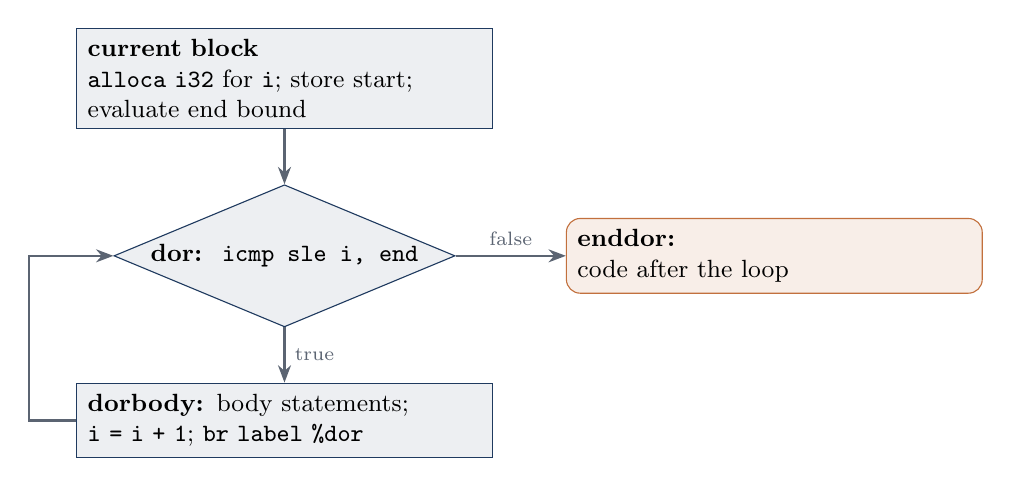
\begin{tikzpicture}[font=\small,node distance=7mm,
  blk/.style={draw=cProcess,fill=cProcess!8,align=left,text width=50mm,inner sep=4pt},
  dec/.style={draw=cProcess,fill=cProcess!8,diamond,aspect=2.4,align=center,inner sep=1pt},
  ex/.style={draw=cResult,fill=cResult!12,rounded corners=5pt,align=left,text width=50mm,inner sep=4pt},
  arr/.style={-{Stealth[length=2.2mm]},cNeutral,thick}]
\node[blk] (init) {\textbf{current block}\\ \fn{alloca i32} for \fn{i}; store start;\\ evaluate end bound};
\node[dec,below=of init] (head) {\textbf{dor:} \ \fn{icmp sle i, end}};
\node[blk,below=of head] (body) {\textbf{dorbody:} body statements;\\ \fn{i = i + 1}; \fn{br label \%dor}};
\node[ex,right=14mm of head] (end) {\textbf{enddor:}\\ code after the loop};
\draw[arr] (init)--(head);
\draw[arr] (head)--node[right,font=\scriptsize]{true}(body);
\draw[arr] (head)--node[above,font=\scriptsize]{false}(end);
\draw[arr] (body.west)--++(-6mm,0)|-(head.west);
\end{tikzpicture}
\caption{Schematic of how \kw{dor} is lowered to LLVM IR: a header block re-tests \fn{i <= end} before every pass and jumps to \fn{enddor} once it fails. The block names come from the IR emitter in \fn{src/kitelang.y}, which adds a number to each label.}
\label{fig:dor}
\end{figure}

\subsection{\kw{palta} -- swap}

\begin{kite}
palta(values[0], values[1]);
palta(score, values[2]);
\end{kite}

\kw{palta} swaps the values of two variables or array elements. Both arguments must be assignable, meaning a variable name or an array element. In LLVM IR it becomes two ordinary loads followed by two stores.

% =====================================================================
\section{Examples and testing}

\subsection{\fn{examples/insertion\_sort.kite}}

This is the main demonstration. It sorts six integers using \kw{dor}, \kw{pecha} and \kw{palta}, then prints them.

\begin{kite}
// KiteLang insertion sort: expected output is 1 2 4 7 8 9.
void insertionSort(int a[], int n) {
    // Adjacent-swap form of insertion sorting, using KiteLang's dor and palta.
    dor (i : 0 -> n - 2) {
        dor (j : 0 -> n - 2 - i) {
            pecha (a[j] > a[j + 1]) {
                palta(a[j], a[j + 1]);
            }
        }
    }
}

int main() {
    int data[6] = {9, 4, 7, 2, 8, 1};
    insertionSort(data, 6);
    dor (i : 0 -> 5) {
        print(data[i]);
    }
    return 0;
}
\end{kite}

\subsection{\fn{examples/array\_smoke.kite}}

A basic test of arrays and \kw{dor}. It prints the array in its original order.

\begin{kite}
int main() {
    int data[6] = {9, 4, 7, 2, 8, 1};
    dor (i : 0 -> 5) {
        print(data[i]);
    }
    return 0;
}
\end{kite}

\begin{shell}
./build/kitelang-interpreter examples/array_smoke.kite
./build/kitelang-compiler examples/array_smoke.kite -o build/smoke.ll
clang build/smoke.ll -o build/smoke && ./build/smoke
\end{shell}

Both should print \fn{9 4 7 2 8 1}, one number per line.

\subsection{Writing your own program}
\begin{enumerate}
\item Create a file, e.g.\ \fn{myprog.kite}, containing an \fn{int main()} function that ends with \fn{return 0;}.
\item Run it with the interpreter: \fn{./build/kitelang-interpreter myprog.kite}.
\item Compile it natively with \fn{./build/kitelang-compiler myprog.kite -o myprog.ll}. Then build it with \fn{clang myprog.ll -o myprog} and run \fn{./myprog}.
\end{enumerate}

\subsection{Automated test}

\begin{shell}
make test
\end{shell}

\fn{make test} does the following:
\begin{enumerate}
\item Builds both phases.
\item Runs the interpreter on \fn{insertion\_sort.kite}, saves the output to \fn{build/interpreter.out}, and compares it with \fn{tests/expected\_insertion\_sort.txt} using \fn{diff -u}.
\item Generates \fn{build/insertion.ll} with the compiler.
\item Builds \fn{build/insertion} with Clang and runs it, saving the output to \fn{build/compiler.out}.
\item Compares that output with the same expected file.
\end{enumerate}

\begin{resultbox}[Expected file \fn{tests/expected\_insertion\_sort.txt}]
\fn{1}, \fn{2}, \fn{4}, \fn{7}, \fn{8}, \fn{9} -- one per line. A zero exit status from \fn{make test} means both phases produced exactly this.
\end{resultbox}

% =====================================================================
\section{Project files}

\begin{longtable}{>{\ttfamily\raggedright}p{0.36\textwidth} >{\raggedright\arraybackslash}p{0.58\textwidth}}
\toprule
\textrm{\textbf{Path}} & \textbf{Purpose}\\
\midrule
\endhead
src/kitelang.l & Flex lexer: keywords, \fn{true}/\fn{false}, identifiers, numbers, operators (\fn{->}, \fn{==}, \fn{!=}, \fn{<=}, \fn{>=}, \fn{\&\&}, \fn{||}), and \fn{//} comments.\\
src/kitelang.y & Bison grammar and AST construction, plus the Phase 1 tree-walking interpreter, the Phase 2 LLVM IR emitter and the shared \fn{main()} driver.\\
src/ast.hpp & AST node kinds and the \fn{Node} structure shared by the parser and the lexer.\\
examples/insertion\_sort.kite & Main Phase 1/Phase 2 sorting demonstration.\\
examples/array\_smoke.kite & Basic array and \kw{dor} loop smoke test.\\
tests/\allowbreak expected\_insertion\_sort.txt & Expected output used by \fn{make test}.\\
Makefile & Build, test and cleanup commands.\\
README.md & Markdown version of this guide.\\
README.pdf & This document.\\
docs/README.tex & LaTeX source of \fn{README.pdf}.\\
docs/generate\_readme.py & Earlier ReportLab script that produced a shorter version of \fn{README.pdf} (kept for reference).\\
KiteLang\_Proposal.pdf & Original Phase 0 language proposal.\\
.gitignore & Excludes \fn{build/}, \fn{*.ll}, \fn{*.o} and other generated files.\\
\midrule
\multicolumn{2}{l}{\textit{Generated by \fn{make} (not committed):}}\\
build/parser.tab.cpp, build/parser.tab.hpp & Parser produced by Bison.\\
build/lex.yy.cpp & Lexer produced by Flex.\\
build/kitelang-interpreter & Phase 1 executable.\\
build/kitelang-compiler & Phase 2 executable.\\
build/insertion.ll, build/insertion & IR and native program produced by \fn{make test}.\\
build/interpreter.out, build/compiler.out & Captured outputs compared by \fn{make test}.\\
\bottomrule
\end{longtable}

% =====================================================================
\newpage
\section{Troubleshooting}

\begin{longtable}{>{\raggedright}p{0.38\textwidth} >{\raggedright\arraybackslash}p{0.56\textwidth}}
\toprule
\textbf{Problem} & \textbf{Fix}\\
\midrule
\endhead
\fn{flex}, \fn{bison} or \fn{clang}: command not found & Install the packages listed in Section~3.\\
\fn{KiteLang syntax error at line N: ...} & Check braces, semicolons and keyword spelling near line \fn{N}.\\
\fn{KiteLang error: undefined name: x} & Declare the variable before using it.\\
\fn{KiteLang error: main function missing} & Add an \fn{int main()} function.\\
\fn{KiteLang error: wrong argument count} & Call the function with the same number of arguments it declares.\\
\fn{array argument must be an array name} & Pass an array parameter as a plain name, e.g.\ \fn{sort(data, 6)}.\\
Clang rejects \fn{ptr} in the \fn{.ll} file & Your Clang is older than 15; see the Clang version box in Section~3.\\
Wrong values or crashes with arrays & Use valid zero-based indexes inside the declared size.\\
Permission denied running a native program & Run \fn{chmod +x build/insertion} and try again.\\
\bottomrule
\end{longtable}

% =====================================================================
\section{Scope and known limitations}

The project targets integer algorithm programs written in one source file. It supports functions, recursion, fixed one-dimensional arrays, conditions, loops and swap. Pointers, dynamic memory, multidimensional arrays, structs/classes, external libraries and multi-file programs are outside the scope.

\begin{warnbox}[Phase 2 (LLVM) back-end limits]
The interpreter handles the whole language. The IR emitter is narrower. To make sure a program compiles with Clang:
\begin{itemize}[leftmargin=*]
\item Write conditions in \kw{pecha}/\kw{dheel} as one comparison, e.g.\ \fn{a > b} or \fn{x != 0}. The emitter does not lower \fn{\&\&}, \fn{||}, \fn{!} or unary \fn{-} correctly, so only use them with the interpreter. Write \fn{0 - x} instead of \fn{-x}.
\item Declare arrays with a literal size, e.g.\ \fn{int a[6];}.
\item Do not store a comparison result directly in a variable (\fn{int c = a < b;}). Use it only as a condition.
\end{itemize}
Both example programs stay within these rules.
\end{warnbox}

\end{document}
